\section{Mudança de frequência de amostragem}

\begin{frame}%[allowframebreaks]
  \frametitle{Mudança da Frequência de Amostragem}
  Muitas vezes é necessário mudar a frequência de amostragem de um sinal
  \begin{itemize}
  \item downsample / decimate
  \item upsample / zero pad
  \item reamostragem
  \item fatores inteiros / racionais
  \item interpolação
  \end{itemize}

  Representação de um sinal contínuo através de um sinal discreto (sequencia de amostras).
  \begin{equation}
   x[n] = x_c (nT)
  \end{equation}

  Muitas vezes é necessário alterar a frequência de amostragem de um sinal.
  \begin{equation}
   x'[n] = x_c(nT')
  \end{equation}
  onde $T'\neq T$

  Embora seja sempre possível reconstruir um sinal contínuo limitado em frequência e
  realizar uma nova amostragem deste sinal, queremos um processamento puramente discreto.
\end{frame}


\subsection{Downsampling}
\begin{frame}[allowframebreaks]
  \frametitle{Downsample por um fator inteiro}
  Podemos reduzir a frequência de amostragem de uma sequência `amostrando'-a e assim
  gerando uma nova sequência.

  Reduzir a frequência de amostragem por um fator $M$
  \begin{equation}
   x_d[n] = x[nM] = x_c(nMT)
  \end{equation}

        \begin{figure}[h!]
        \centering
        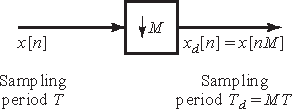
\includegraphics[width=0.4\textwidth]{images/fig419.pdf}
        \caption{Representação de um compressor ou amostrador discreto. \citep{oppenheim2009}.}
        \label{fig:fig419}
        \end{figure}

  A transformada discreta de Fourier de $x[n] = x_c(nT)$ é
  \begin{equation}
  X(e^{j\omega}) = \frac{1}{T} \sum_{k=-\infty}^{\infty} X_c \left( j \left( \frac{\omega}{T} - \frac{2 \pi k}{T} \right) \right) .
  \end{equation}

  A transformada discreta de Fourier de $x_d[n] = x[nM] = x_c(nT')$, onde $T'=MT$, é
  \begin{align}
   X_d(e^{j\omega}) &= \frac{1}{T'} \sum_{k=-\infty}^{\infty} X_c \left( j \left( \frac{\omega}{T'} - \frac{2 \pi k}{T'} \right) \right) \\
                    &= \frac{1}{MT}  \sum_{k=-\infty}^{\infty} X_c \left( j \left( \frac{\omega}{MT} - \frac{2 \pi k}{MT} \right) \right)
  \end{align}

  \framebreak
  Podemos fazer o índice do somatório da seguinte forma
  \begin{equation}
  r = i + kM
  \end{equation}
  onde $k$ e $i$ são inteiros tais que $-\infty < k < \infty$ e $0 \leq i \leq M-1$.
  Podemos assim reescrever a equação anterior na seguinte forma:
  \begin{align}
  X_d(e^{j\omega}) &= \frac{1}{M} \sum_{i=0}^{M-1} \left[ \frac{1}{T} \sum_{k=-\infty}^{\infty} X_c \left( j \left( \frac{\omega}{MT} - \frac{2 \pi k}{T} - \frac{2\pi i}{MT} \right) \right)  \right] \\
                   &= \frac{1}{M} \sum_{i=0}^{M-1} X\left( e^{j(\omega - 2\pi i)/M} \right) .
  \end{align}
  Teremos $M$ cópias de $X(e^{j\omega})$ dilatadas por um fator $M$ e transladadas por $2\pi i/M$.


  Não haverá \textit{aliasing} se $X(e^{j\omega})$ for limitado em frequência
  \begin{equation}
  X(e^{j\omega}) = 0 , \quad \omega_N \leq \vert \omega \vert \leq \pi,
  \end{equation}
  e $2\pi/M \geq 2 \omega_N$.

        \begin{figure}[h!]
        \centering
        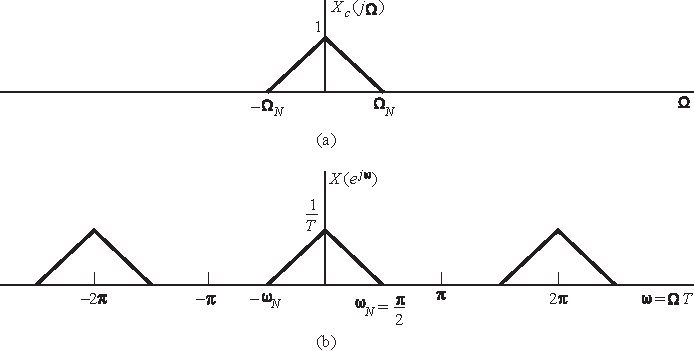
\includegraphics[width=0.75\textwidth]{images/fig421ab.pdf}
        %\caption{Transformada de Fourier de um sinal limitado em frequência. \cite{oppenheim2009}).}
        \label{fig:fig421ab}
        \end{figure}

        \begin{figure}[h!]
        \centering
        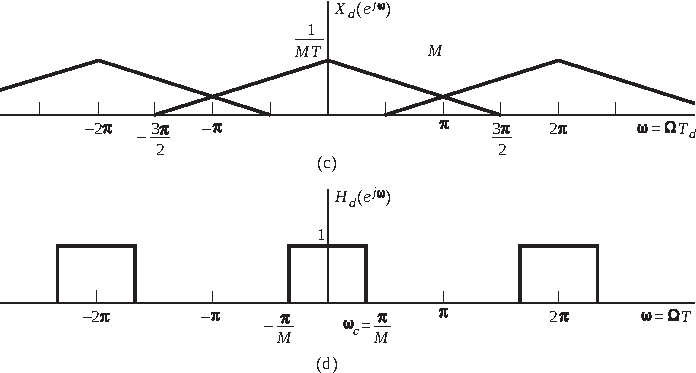
\includegraphics[width=0.75\textwidth]{images/fig421cd.pdf}
        %\caption{Transformada de Fourier de um sinal limitado em frequência. \cite{oppenheim2009}).}
        \label{fig:fig421cd}
        \end{figure}

        \begin{figure}[h!]
        \centering
        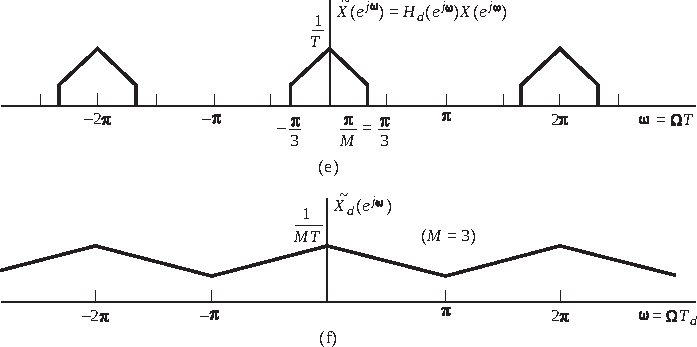
\includegraphics[width=0.75\textwidth]{images/fig421ef.pdf}
        %\caption{Transformada de Fourier de um sinal limitado em frequência. \cite{oppenheim2009}).}
        \label{fig:fig421ef}
        \end{figure}


  \framebreak
  De forma geral, para evitar \textit{aliasing} ao realizar um \textit{downsample} por um fator $M$
  é necessário que
  \begin{equation}
  \omega_N M \leq \pi \quad \quad \textmd{ ou } \quad \quad \omega_N \leq \pi/M.
  \end{equation}

        \begin{figure}[h!]
        \centering
        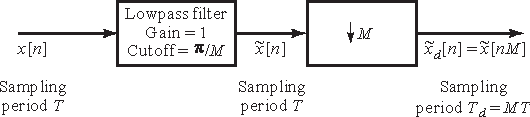
\includegraphics[width=0.65\textwidth]{images/fig422.pdf}
        \caption{Sistema geral para redução da frequência de amostragem por um fator $M$. \citep{oppenheim2009}.}
        \label{fig:fig422}
        \end{figure}

\end{frame}


\subsection{Upsampling}
\begin{frame}[allowframebreaks]
  \frametitle{upsample por um fator inteiro}

  Considere o sinal $x[n]$ o qual queremos aumentar a frequência de amostragem por um fator $L$.

  Vamos considerar o sinal contínuo subjacente $x_c(t)$. O objetivo é obter as amostras
  \begin{equation}
   x_i[n] = x_c(nT')
  \end{equation}
  onde $T'=T/L$, a partir das amostras
  \begin{equation}
   x[n] = x_c(nT .)
  \end{equation}
  Das equações acima, segue que
  \begin{equation}
   x_i[n] = x[n/L] = x_c(nT/L), \quad 0, \pm L, \pm 2 L, \ldots
  \end{equation}

  \framebreak
  Sistema para aumentar a frequência de amostragem por um fator $L$.
        \begin{figure}[h!]
        \centering
        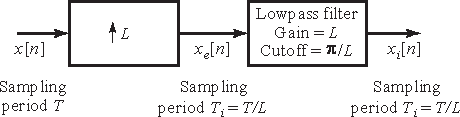
\includegraphics[width=0.65\textwidth]{images/fig423.pdf}
        \caption{Sistema geral para aumentar a frequência de amostragem por um fator $L$. \citep{oppenheim2009}.}
        \label{fig:fig423}
        \end{figure}

  O sistema da esquerda é chamado expansor. Sua saída será
  \begin{equation}
   x_e[n] = \begin{cases} 
      x[n/L] , \quad n = 0, \pm L, \pm 2L, \ldots \\
      0 , \quad \text{ caso contrário,}
            \end{cases}
  \end{equation}
  ou de forma equivalente,
  \begin{equation}
   x_e[n] = \sum_{k=-\infty}^{\infty} x[k] \delta[n-kL] .
  \end{equation}

  A transformada de Fourier de $x_e[n]$ pode ser expressa como
  \begin{align}
   X_e(e^{j\omega}) &= \sum_{n=-\infty}^{\infty} \left( \sum_{k=-\infty}^{\infty} x[k] \delta[n-kL]  \right) e^{-j\omega n} \\
                    &= \sum_{k=-\infty}^{\infty} x[k] e^{-j\omega L k} = X(e^{j\omega L})
  \end{align}
  Ou seja, $X_e(e^{j\omega})$ é obtido através de $X(e^{j\omega})$ por uma compressão de fator $L$.

  $X_i(e^{j\omega})$ pode ser obtido a partir de $X_e(e^{j\omega})$ realizando a correção da
  amplitude de $1/T$ para $1/T'$ e removendo todas as réplicas escalonadas de $X_c(j\Omega)$,
  exceto aquelas nos múltiplos de $2\pi$.

        \begin{figure}[h!]
        \centering
        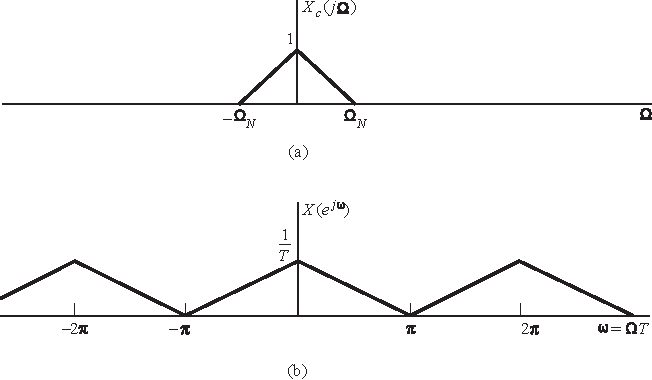
\includegraphics[width=0.65\textwidth]{images/fig424ab.pdf}
        %\caption{Sistema geral para aumentar a frequencia de amostragem por um fator $L$. \cite{oppenheim2009}.}
        \label{fig:fig424ab}
        \end{figure}

        \begin{figure}[h!]
        \centering
        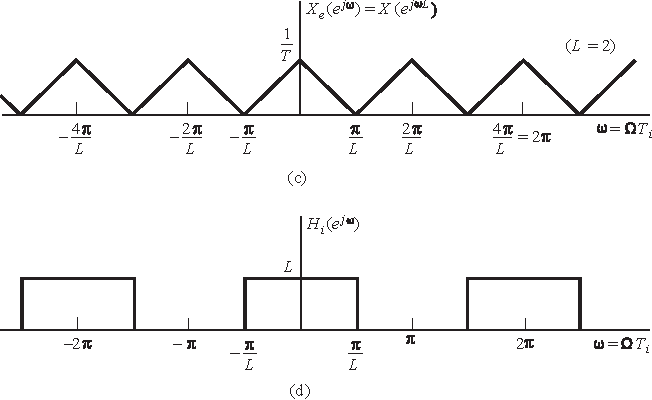
\includegraphics[width=0.65\textwidth]{images/fig424cd.pdf}
        %\caption{Sistema geral para aumentar a frequencia de amostragem por um fator $L$. \cite{oppenheim2009}.}
        \label{fig:fig424cd}
        \end{figure}

        \begin{figure}[h!]
        \centering
        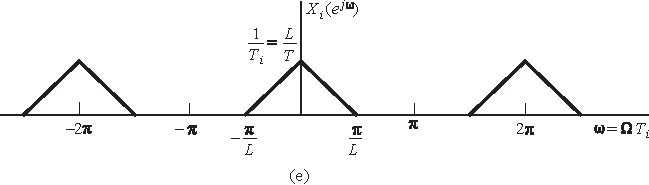
\includegraphics[width=0.65\textwidth]{images/fig424e.pdf}
        %\caption{Sistema geral para aumentar a frequencia de amostragem por um fator $L$. \cite{oppenheim2009}.}
        \label{fig:fig424e}
        \end{figure}

  O interpolador será um filtro passa-baixas com frequência de corte $\pi/L$ e ganho $L$.
  Sua resposta ao impulso será
  \begin{equation}
  h_i[n] = \frac{\sin (\pi n /L)}{\pi n/L} .
  \end{equation}
  Obteremos então
  \begin{equation}
  x_i[n] = \sum_{k=-\infty}^{\infty} x[k] \frac{\sin[\pi(n-kL)/L]}{\pi (n-kL)/L}
  \end{equation}

  Note que $h_i[n]$ possui as seguintes propriedades
  \begin{align}
   h_i[0] &= 1, \\
   h_i[n] &= 0,     \quad n = \pm L, \pm 2L, \ldots 
  \end{align}
  Teremos assim
  \begin{equation}
   x_i[n] = x[n/L] = x_c(nT/L) = x_c(nT'), \quad n = 0, \pm L, \pm 2L, \ldots
  \end{equation}

\end{frame}


\subsubsection{Interpolador Linear}
\begin{frame}[allowframebreaks]
  \frametitle{Interpolador Linear}

  Apenas a título de comparação, vamos analisar um outro interpolador muito comum: o interpolador linear.
  
  Resposta ao impulso de um interpolador linear:
  \begin{equation}
    h_{\text{lin}} = \begin{cases}
         1 - \vert n \vert / L, & \vert n \vert \leq L , \\
         0, &\text{caso contrário.}
                    \end{cases}
  \end{equation}

  A saída do filtro interpolador será
  \begin{equation}
   x_{\text{lin}} [n] = \sum_{k=n-L+1}^{n+L-1} x_e[k] h_{\text{lin}}[n-k] .
  \end{equation}
  onde $x_e[n]$ é a saída de um \textit{upsample} por um fator $L$.
  Note que as amostras originais são preservadas pois $h_{\text{lin}}[0] = 1$
  e $h_{\text{lin}}[n]=0$ para $|n| \geq L$.

  A resposta em frequência do interpolador linear é dada por
  \begin{equation}
   H_{\text{lin}} (e^{j\omega}) = \frac{1}{L} \left[ \frac{\sin (\omega L/2)}{\sin (\omega /2)} \right]^2 .
  \end{equation}


  \framebreak

  Para $L=5$ teremos o seguinte exemplo.
        \begin{figure}[h!]
        \centering
        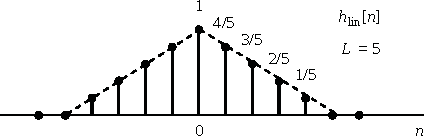
\includegraphics[width=0.5\textwidth]{images/fig425.pdf}
        \caption{Resposta ao impulso do interpolador linear com $L=5$. \citep{oppenheim2009}.}
        \label{fig:fig425}
        \end{figure}

        \begin{figure}[h!]
        \centering
        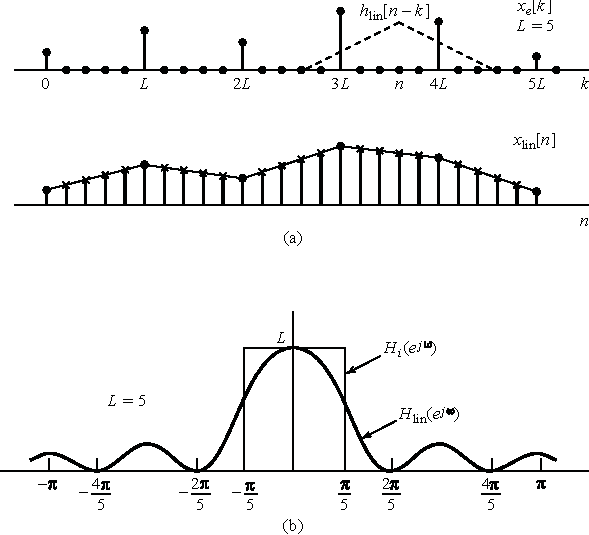
\includegraphics[width=0.45\textwidth]{images/fig426.pdf}
        \caption{Filtragem com o interpolador linear e sua resposta em frequência. \citep{oppenheim2009}.}
        \label{fig:fig426}
        \end{figure}
\end{frame}



\subsection{Mudança da frequência de amostragem por um fator não inteiro}
\begin{frame}[allowframebreaks]
  \frametitle{Mudança da frequência de amostragem por um fator não inteiro}

        \begin{figure}[h!]
        \centering
        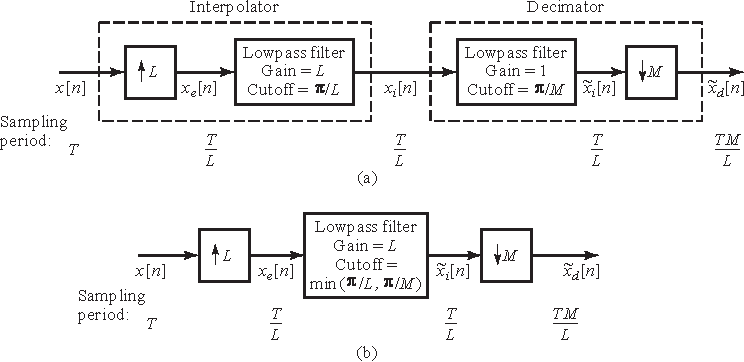
\includegraphics[width=0.75\textwidth]{images/fig429.pdf}
        \caption{Sistema para mudar a frequência de amostragem por um fator não inteiro. \citep{oppenheim2009}.}
        \label{fig:fig429}
        \end{figure}
  \framebreak

  \begin{example}[Mudança da frequência de amostragem por um fator nao inteiro]
  Suponha um sinal $X_c(j\Omega)$ limitado em frequência, conforme ilustrado.
  Este sinal é amostrado à taxa de Nyquist, $2\pi/T = 2\Omega_N$. A DTFT resultante é
  \begin{equation}
  X(e^{j\omega}) = \frac{1}{T} \sum_{k=-\infty}^{\infty} X_c \left( j \left( \frac{\omega}{T} - \frac{2\pi k}{T} \right) \right)
  \end{equation}
  também ilustrado abaixo. Para mudar o período de amostragem para $(3/2)T$, iremos primeiramente interpolar por
  um fator $L=2$ e depois decimar por um fator $M=3$.

  \examplebreak

        \begin{figure}[h!]
        \centering
        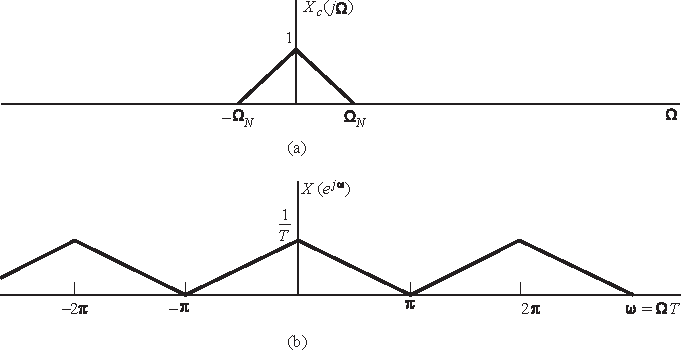
\includegraphics[width=0.6\textwidth]{images/fig430ab.pdf}
        %\caption{Sistema para mudar a frequência de amostragem por um fator nao inteiro. \cite{oppenheim2009}.}
        \label{fig:fig430ab}
        \end{figure}

  \examplebreak

        \begin{figure}[h!]
        \centering
        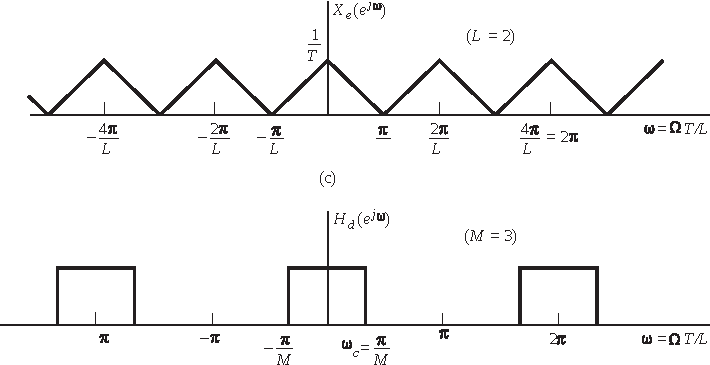
\includegraphics[width=0.6\textwidth]{images/fig430cd.pdf}
        %\caption{Sistema para mudar a frequência de amostragem por um fator nao inteiro. \cite{oppenheim2009}.}
        \label{fig:fig430cd}
        \end{figure}

  \examplebreak

        \begin{figure}[h!]
        \centering
        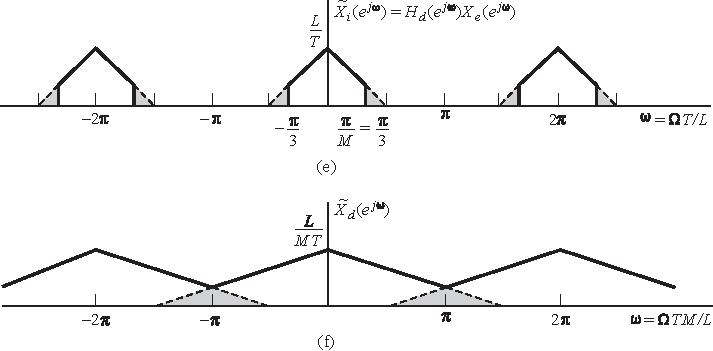
\includegraphics[width=0.6\textwidth]{images/fig430ef.pdf}
        %\caption{Sistema para mudar a frequência de amostragem por um fator nao inteiro. \cite{oppenheim2009}.}
        \label{fig:fig430ef}
        \end{figure}

  \end{example}
\end{frame}

\begin{frame}%[allowframebreaks]
  \frametitle{Resample}

  \centering
  
\includegraphics[width=0.3\textwidth]{images/qrcode-jupyter-resampling.pdf}
  \url{https://nbviewer.jupyter.org/github/leolca/notebooks/blob/master/aev/resample.ipynb}

\end{frame}



\subsection{Processamento Multi-taxa de Sinais}
\begin{frame}[allowframebreaks]
  \frametitle{Processamento Multi-taxa de Sinais}
  O processamento de sinais a multi-taxas refere-se à utilização de \textit{upsampling},
  \textit{downsampling}, compressores e expansores em uma variedade de maneiras para
  aumentar a eficiência do sistema de processamento de sinais.
\end{frame}

\begin{frame}[allowframebreaks]
  \frametitle{Intercâmbio entre filtro e downsampling/upsampling}

        \begin{figure}[h!]
        \centering
        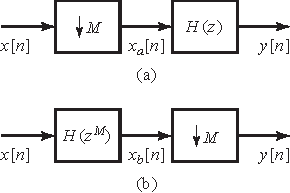
\includegraphics[width=0.4\textwidth]{images/fig431.pdf}
        \caption{Dois sistemas equivalentes, com base nas identidades do \textit{downsample}. \citep{oppenheim2009}.}
        \label{fig:fig431}
        \end{figure}

  Analisando o sistema (b) temos:
  \begin{equation}
   X_b(e^{j\omega}) = H(e^{j\omega M}) X(e^{j \omega})
  \end{equation}
  e
  \begin{equation}
   Y(e^{j \omega}) = \frac{1}{M} \sum_{i=0}^{M-1} X_b \left( e^{j (\omega / M - 2\pi i/M)} \right).
  \end{equation}
  logo
  \begin{equation}
   Y(e^{j \omega}) = \frac{1}{M} \sum_{i=0}^{M-1} X\left( e^{j (\omega / M - 2\pi i/M)} \right) H\left( e^{j(\omega - 2\pi i)} \right).
  \end{equation}
  Como $H\left( e^{j(\omega - 2\pi i)} \right) = H(e^{j\omega})$, poderemos simplificar, ficando
  \begin{align}
   Y(e^{j \omega}) &= H(e^{j\omega}) \frac{1}{M} \sum_{i=0}^{M-1} X\left( e^{j (\omega / M - 2\pi i/M)} \right) \\
                &= H(e^{j\omega}) X_a(e^{j\omega}) ,
  \end{align}
  o que corresponde ao sistema (a) da figura.


  \framebreak

        \begin{figure}[h!]
        \centering
        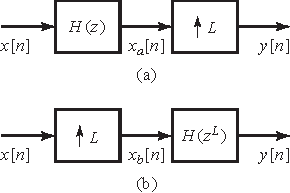
\includegraphics[width=0.4\textwidth]{images/fig432.pdf}
        \caption{Dois sistemas equivalentes, com base nas identidades do \textit{upsample}. \citep{oppenheim2009}.}
        \label{fig:fig432}
        \end{figure}

  \begin{align}
   Y(e^{j\omega}) &= X_a (e^{j\omega L})  \\
                  &= X(e^{j\omega L}) H(e^{j\omega L}) 
  \end{align}
  \begin{equation}
   X_b(e^{j\omega}) = X(e^{j\omega L})
  \end{equation}
  \begin{equation}
   Y(e^{j\omega}) = H(e^{j\omega L}) X_b(e^{j\omega})
  \end{equation}

\end{frame}


\subsection{Decimação e Interpolação com múltiplos estágios}
\begin{frame}[allowframebreaks]
  \frametitle{Decimação e Interpolação com múltiplos estágios}
  Quando a decimação e interpolação envolvem fatores grandes, utiliza-se filtros com resposta ao 
  impulso longa. É possível reduzir significativamente o custo computacional utilizando 
  múltiplos estágios.

  \framebreak 

        \begin{figure}[h!]
        \centering
        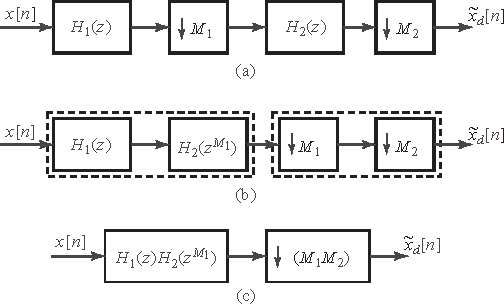
\includegraphics[width=0.65\textwidth]{images/fig433.pdf}
        \caption{Decimação em múltiplos estágios. \citep{oppenheim2009}.}
        \label{fig:fig433}
        \end{figure}

  O fator final de decimação é $M = M_1 M_2$. Para realizar a decimação pelo fato $M$
  seria necessário um filtro com frequência de corte $\nicefrac{\pi}{M} = \nicefrac{\pi}{M_1 M_2}$.
  Este filtro é bem mais estreito que os filtros $H_1(z)$ e $H_2(z)$ com frequência de corte
  $\nicefrac{\pi}{M_1}$ e $\nicefrac{\pi}{M_2}$, respectivamente. Filtros com banda mais estreita 
  requerem sistemas de ordem maior para obter transição mais abrupta. Desta forma, a implementação
  em dois estágios será mais eficiente.


        \begin{figure}[h!]
        \centering
        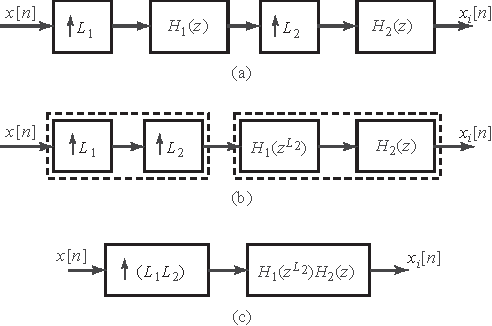
\includegraphics[width=0.55\textwidth]{images/fig434.pdf}
        \caption{Interpolação em múltiplos estágios. \citep{oppenheim2009}.}
        \label{fig:fig434}
        \end{figure}

\end{frame}


\subsection{Decomposição Polifásica}
\begin{frame}[allowframebreaks]
  \frametitle{Decomposição Polifásica}

  A resposta ao impulso $h[n]$ pode ser decomposta em $M$ subsequentes $h_k[n]$.
  \begin{equation}
   h_k[n] = \begin{cases}
             h[n+k] , & n=\text{múltiplo inteiro de }M, \\
                0,    & \text{caso contrário.}
            \end{cases}
  \end{equation}

  \begin{equation}
   h[n] = \sum_{k=0}^{M-1} h_k [n-k]
  \end{equation}

  \framebreak

        \begin{figure}[h!]
        \centering
        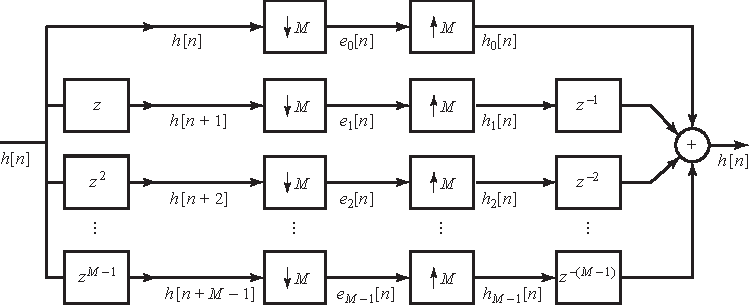
\includegraphics[width=0.65\textwidth]{images/fig435.pdf}
        \caption{Decomposição polifásica de $h[n]$ usando as componentes $e_k[n]$. \citep{oppenheim2009}.}
        \label{fig:fig435}
        \end{figure}
  
  As sequências $e_k[n]$ são dadas por
  \begin{equation}
   e_k[n] = h[nM+k] = h_k[nM]
  \end{equation}
  e são chamadas de componentes polifásicas de $h[n]$.

  \framebreak

        \begin{figure}[h!]
        \centering
        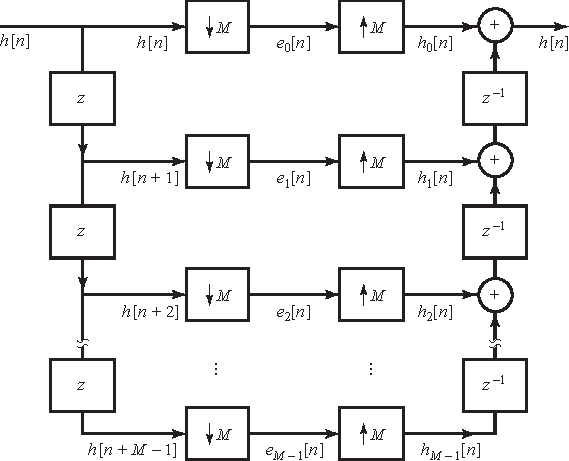
\includegraphics[width=0.45\textwidth]{images/fig436.pdf}
        \caption{Representação com atrasos em cadeia. \citep{oppenheim2009}.}
        \label{fig:fig436}
        \end{figure}

  \framebreak

  Representando no domínio da frequência ou no domínio z, teremos
  \begin{align}
   Z\{ h[n] \} &= Z\{  \sum_{k=0}^{M-1} h_k [n-k] \} \\
          H(z) &= \sum_{k=0}^{M-1} Z\{ h_k [n-k] \} \\
               &= \sum_{k=0}^{M-1} Z\{ h_k [n] \} z^{-k} \\
               &= \sum_{k=0}^{M-1} E_k(z^M) z^{-k}
  \end{align}
  onde utilizamos o fato de que $e_k[n]=h_k[nM]$.

  \framebreak 

  Representamos então $H(z)$ como uma soma de filtros polifásico atrasados.


        \begin{figure}[h!]
        \centering
        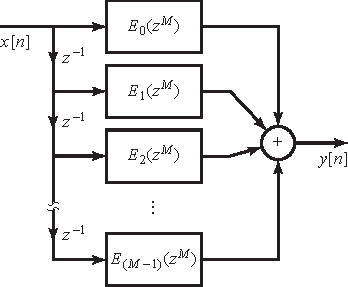
\includegraphics[width=0.4\textwidth]{images/fig437.pdf}
        \caption{Estrutura da decomposição polifásica de $h[n]$. \citep{oppenheim2009}.}
        \label{fig:fig437}
        \end{figure}
\end{frame}


\subsection{Implementação de decimadores usando decomposição polifásica}
\begin{frame}[allowframebreaks]
  \frametitle{Implementação de decimadores usando decomposição polifásica}

  Uma aplicação importante da decomposição polifásica é na implementação de filtros
  cuja saída é seguida por um \textit{downsample} (note que $1$ em cada $M$ amostras
  geradas pelo filtro é mantida e as demais $M-1$ são descartadas).

        \begin{figure}[h!]
        \centering
        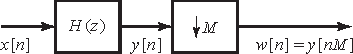
\includegraphics[width=0.4\textwidth]{images/fig438.pdf}
        \caption{Sistema de decimadão. \citep{oppenheim2009}.}
        \label{fig:fig438}
        \end{figure}

  Suponha que $H(z)$ é um filtro FIR com $N$ pontos. Serão necessárias $N$ multiplicações 
  e $(N-1)$ adições por unidade de tempo para calcular a saída.

  Suponha que $h[n]$ seja expresso em componentes polifásicas
  \begin{equation}
   e_k[n] = h[nM+k]
  \end{equation}
  e assim podemos representar $H(z)$ como
  \begin{equation}
   H(z) = \sum_{k=0}^{M-1} E_k (z^M) z^{-k} 
  \end{equation} 

        \begin{figure}[h!]
        \centering
        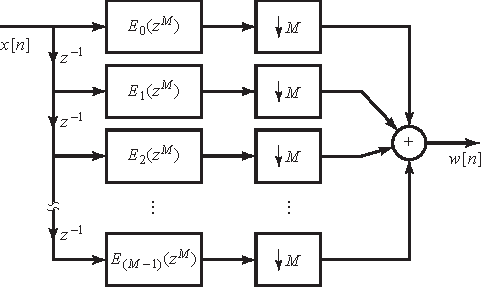
\includegraphics[width=0.55\textwidth]{images/fig439.pdf}
        \caption{Implementação utilizando decomposição polifásicas. \citep{oppenheim2009}.}
        \label{fig:fig439}
        \end{figure}

        \begin{figure}[h!]
        \centering
        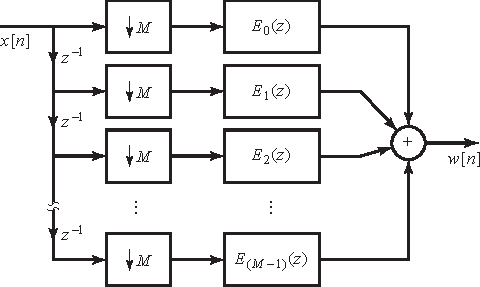
\includegraphics[width=0.55\textwidth]{images/fig440.pdf}
        \caption{Implementação após utilizar a identidade do \textit{downsapling}. \citep{oppenheim2009}.}
        \label{fig:fig440}
        \end{figure}

  Os filtros $E_k(z)$ possuem comprimento $N/M$ e estão a uma taxa $1/M$ em relação ao original.
  Consequentemente, cada filtro fará $\frac{1}{M}\left(\frac{N}{M}\right)$ multiplicações 
  e $\frac{1}{M}\left(\frac{N}{M}-1\right)$ adições por unidade de tempo. Como são $M$ componentes 
  polifásicas o sistema requererá $N/M$ multiplicações e $\left(\frac{N}{M}-1\right)+(M-1)$ adições
  por unidade de tempo.

\end{frame}


\subsection{Implementação de interpoladores usando decomposição polifásica}
\begin{frame}[allowframebreaks]
  \frametitle{Implementação de interpoladores usando decomposição polifásica}

        \begin{figure}[h!]
        \centering
        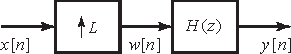
\includegraphics[width=0.55\textwidth]{images/fig441.pdf}
        \caption{Sistema de interpolação. \citep{oppenheim2009}.}
        \label{fig:fig441}
        \end{figure}

        \begin{figure}[h!]
        \centering
        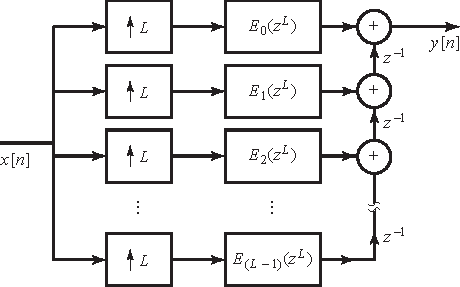
\includegraphics[width=0.55\textwidth]{images/fig442.pdf}
        \caption{Decomposição polifásica do filtro de interpolação. \citep{oppenheim2009}.}
        \label{fig:fig442}
        \end{figure}

        \begin{figure}[h!]
        \centering
        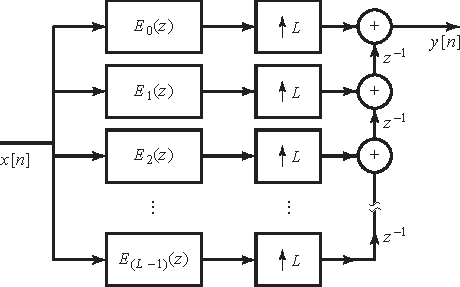
\includegraphics[width=0.55\textwidth]{images/fig443.pdf}
        \caption{Implementação usando a identidade do \textit{upsample}. \citep{oppenheim2009}.}
        \label{fig:fig443}
        \end{figure}

\end{frame}


\begin{frame}%[allowframebreaks]
  \frametitle{Notebook - implementação polifásica}
    \centering
      
\includegraphics[width=0.4\textwidth]{images/qrcode-jupyter-polyphase.pdf}

      \url{https://nbviewer.jupyter.org/github/leolca/notebooks/blob/master/aev/polyphase.ipynb}
\end{frame} 


\subsection{Banco de Filtros Multi taxa}
\begin{frame}[allowframebreaks]
  \frametitle{Banco de Filtros Multi taxa}

        \begin{figure}[h!]
        \centering
        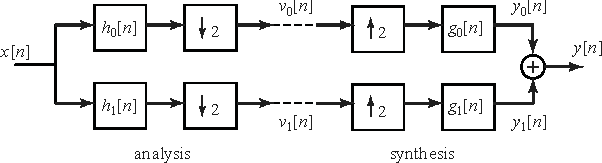
\includegraphics[width=0.75\textwidth]{images/fig444.pdf}
        \caption{Banco de filtro de análise e síntese com dois canais. \citep{oppenheim2009}.}
        \label{fig:fig444}
        \end{figure}


  A decomposição requer que $h_0[n]$ e $h_1[n]$ sejam filtros passa-baixa e passa-alta 
  respectivamente. Uma abordagem comum é obter o filtro passa-alta a partir do filtro
  passa-baixa fazendo $h_1[n] = e^{j\pi n} h_0[n]$. Isto implica em $H_1(e^{j\omega}) = H_0(e^{j(\omega - \pi)})$.

  Analisando a figura, queremos
  \begin{align}\label{eq-yejw-fb}
  Y(e^{j\omega}) &= \frac{1}{2} \left[ G_0(e^{j\omega}) H_0(e^{j\omega}) + G_1(e^{j\omega}) H_1(e^{j\omega}) \right] X(e^{j\omega}) \\
                & + \frac{1}{2} \left[ G_0(e^{j\omega}) H_0(e^{j(\omega-\pi)}) + G_1(e^{j\omega}) H_1(e^{j(\omega-\pi)}) \right] X(e^{j(\omega - \pi)}) .
  \end{align}

  Note que teremos reconstrução perfeita se os filtros forem ideais, entretanto também é possível 
  obter reconstrução perfeita com filtros não ideias, para tanto o \textit{aliasing} deverá ocorrer.
  Note que o segundo termo da expressão para $Y(e^{j\omega})$ representa a potencial distorção por
  \textit{aliasing}. Este termo poderá ser eliminado escolhendo
  \begin{equation}
  G_0(e^{j\omega}) H_0(e^{j(\omega-\pi)}) + G_1(e^{j\omega}) H_1(e^{j(\omega-\pi)}) = 0.
  \end{equation}
  Esta condição para cancelamento do \textit{aliasing} é satisfeita, por exemplo, pelo conjunto de condições:
  \begin{align}
  h_1[n] = e^{j\pi n} h_0[n]    & \Longleftrightarrow H_1(e^{j\omega}) = H_0(e^{j(\omega-\pi)})  \\
  g_0[n] = 2 h_0[n]             & \Longleftrightarrow G_0(e^{j\omega}) =  2 H_0(e^{j\omega}) \\
  g_1[n] = -2 h_1[n]            & \Longleftrightarrow G_1(e^{j\omega}) =  -2 H_0(e^{j(\omega-\pi)}) 
  \end{align}
  Os filtros $h_0[n]$ e $h_1[n]$ são chamados filtros espelhados em quadratura pois eles devem possuir simetria 
  em torno de $\omega = \pi/2$. Usando as condições acima, \cref{eq-yejw-fb} ficará da forma
  \begin{equation}
  Y(e^{j\omega}) = \left[ H_0^2(e^{j\omega}) - H_0^2(e^{j(\omega-\pi)}) \right] X(e^{j\omega}) ,
  \end{equation}
  e assim concluímos que a reconstrução perfeita (com possível atraso de $M$ amostras) requererá 
  \begin{equation}
  H_0^2(e^{j\omega}) - H_0^2(e^{j(\omega-\pi)})  = e^{-j\omega M} .
  \end{equation}
  Os únicos filtros computacionalmente realizáveis capazes de fornecer uma reconstrução exata são
  aqueles com resposta ao impulso da forma
  \begin{equation}
  h_0[n] = c_0 \delta[n-2n_0] + c_1 \delta[n-2n_1 - 1],  
  \end{equation}
  onde $n_0$ e $n_1$ são inteiros arbitrários e $c_0 c_1 = \nicefrac{1}{4}$.

  Por exemplo, considere
  \begin{equation}
  h_0[n] = \frac{1}{2} (\delta[n] + \delta[n-1]) ,
  \end{equation}
  com resposta em frequência 
  \begin{equation}
  H_0(e^{j\omega}) = \cos(\omega/2) e^{-j\omega} .
  \end{equation}
  Para este exemplo, teremos $Y(e^{j\omega}) = e^{-j\omega} X(e^{j\omega})$.

  Podemos empregar a decomposição polifásica a este banco de filtros. 
  %%% fig 445(a)
        \begin{figure}[h!]
        \centering
        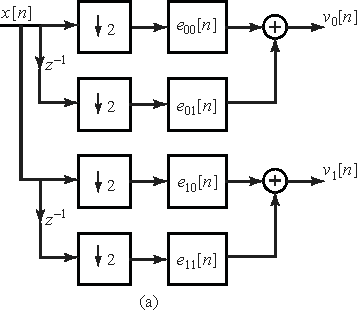
\includegraphics[width=0.4\textwidth]{images/fig445a.pdf}
        \caption{Representação polifásica do banco de filtros de análise. \citep{oppenheim2009}.}
        \label{fig:fig445a}
        \end{figure}


  Usando as relações
  \begin{align}
  e_{00}[n] &= h_0[2n] \\
  e_{01}[n] &= h_0[2n+1] \\
  e_{10}[n] &= h_1[2n] = e^{j2\pi n} h_0[2n] = e_{00}[n] \\
  e_{11}[n] &= h_1[2n+1] = e^{j2\pi n} e^{j\pi} h_0[2n+1] = -e_{01}[n] .
  \end{align}
  Logo poderemos representar o banco de filtros utilizando metade dos cálculos computacionais.
  %%% fig 445(b)
        \begin{figure}[h!]
        \centering
        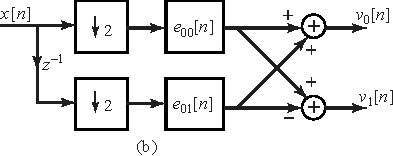
\includegraphics[width=0.4\textwidth]{images/fig445b.pdf}
        \caption{Representação simplificada. \citep{oppenheim2009}.}
        \label{fig:fig445b}
        \end{figure}


  O mesmo pode ser feito com o filtro de síntese. Assim teremos o sistema conforme ilustrado.
  %%% fig 446
        \begin{figure}[h!]
        \centering
        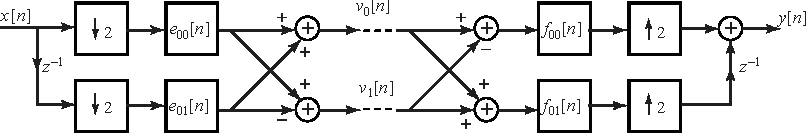
\includegraphics[width=0.85\textwidth]{images/fig446.pdf}
        \caption{Representação polifásica do banco de filtros de análise e síntese. \citep{oppenheim2009}.}
        \label{fig:fig446}
        \end{figure}

\end{frame}


